% figures.tex - TikZ figures for the book
% Include this file in chapters where figures are needed

% ============================================
% FIGURE: Workflow Compression - Before vs After AI
% ============================================
\newcommand{\figWorkflowCompression}{%
\begin{tikzpicture}[
    node distance=0.8cm,
    box/.style={rectangle, draw=green!60!black, fill=green!10, minimum width=2.2cm, minimum height=0.8cm, align=center, font=\small},
    arrow/.style={-{Stealth[length=2mm]}, thick, draw=gray!70},
    label/.style={font=\small\bfseries, align=center}
]
% Traditional workflow (top)
\node[label] at (0, 2) {Traditional Workflow};
\node[box] (t1) at (-4, 1) {Discovery\\2-4 weeks};
\node[box] (t2) at (-1.5, 1) {Requirements\\1-2 weeks};
\node[box] (t3) at (1, 1) {Design\\1-2 weeks};
\node[box] (t4) at (3.5, 1) {Dev + Test\\4-8 weeks};

\draw[arrow] (t1) -- (t2);
\draw[arrow] (t2) -- (t3);
\draw[arrow] (t3) -- (t4);

% AI-Assisted workflow (bottom)
\node[label] at (0, -0.5) {AI-Assisted Workflow};
\node[box, fill=blue!10, draw=blue!60!black] (a1) at (-3, -1.5) {Prompt\\+ Draft};
\node[box, fill=blue!10, draw=blue!60!black] (a2) at (-0.5, -1.5) {Evaluate\\+ Verify};
\node[box, fill=blue!10, draw=blue!60!black] (a3) at (2, -1.5) {Iterate};
\node[box, fill=blue!10, draw=blue!60!black] (a4) at (4.5, -1.5) {Ship};

\draw[arrow, draw=blue!60] (a1) -- (a2);
\draw[arrow, draw=blue!60] (a2) -- (a3);
\draw[arrow, draw=blue!60] (a3) -- (a4);
\draw[arrow, draw=blue!60, dashed] (a3.south) -- ++(0,-0.3) -| (a1.south);

% Time labels
\node[font=\footnotesize, gray] at (0, 0.3) {Weeks to Months};
\node[font=\footnotesize, blue!60!black] at (0, -2.3) {Days to Weeks};
\end{tikzpicture}%
}

% ============================================
% FIGURE: AI Task Suitability Matrix
% ============================================
\newcommand{\figTaskMatrix}{%
\begin{tikzpicture}[
    scale=0.9,
    cell/.style={minimum width=3.5cm, minimum height=2cm, align=center, font=\small},
    header/.style={font=\small\bfseries}
]
% Axes
\draw[-{Stealth}, thick] (0,0) -- (8,0) node[right, header] {Volume};
\draw[-{Stealth}, thick] (0,0) -- (0,5) node[above, header] {Stakes};

% Quadrant labels
\node[cell, fill=green!20] at (2, 1.2) {High AI\\Low Verify\\\\Drafts, brainstorms,\\clustering};
\node[cell, fill=yellow!20] at (6, 1.2) {High AI\\Medium Verify\\\\Summaries, reports,\\documentation};
\node[cell, fill=orange!20] at (2, 3.5) {Low AI\\High Verify\\\\Strategy decisions,\\sensitive comms};
\node[cell, fill=red!20] at (6, 3.5) {Selective AI\\Rigorous Verify\\\\Customer-facing,\\legal, financial};

% Axis labels
\node[font=\footnotesize] at (2, -0.4) {Low};
\node[font=\footnotesize] at (6, -0.4) {High};
\node[font=\footnotesize, rotate=90] at (-0.4, 1.2) {Low};
\node[font=\footnotesize, rotate=90] at (-0.4, 3.5) {High};
\end{tikzpicture}%
}

% ============================================
% FIGURE: The Jagged Frontier
% ============================================
\newcommand{\figJaggedFrontier}{%
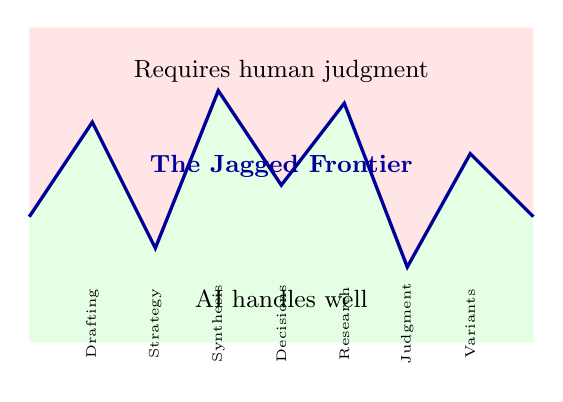
\begin{tikzpicture}[scale=0.8]
% Draw jagged line representing AI capability
\draw[very thick, blue!60!black] 
    (0, 2) -- (1, 3.5) -- (2, 1.5) -- (3, 4) -- (4, 2.5) -- (5, 3.8) -- (6, 1.2) -- (7, 3) -- (8, 2);

% Shade above and below
\fill[green!10] (0,0) -- (0, 2) -- (1, 3.5) -- (2, 1.5) -- (3, 4) -- (4, 2.5) -- (5, 3.8) -- (6, 1.2) -- (7, 3) -- (8, 2) -- (8, 0) -- cycle;
\fill[red!10] (0, 2) -- (1, 3.5) -- (2, 1.5) -- (3, 4) -- (4, 2.5) -- (5, 3.8) -- (6, 1.2) -- (7, 3) -- (8, 2) -- (8, 5) -- (0, 5) -- cycle;

% Redraw line on top
\draw[very thick, blue!60!black] 
    (0, 2) -- (1, 3.5) -- (2, 1.5) -- (3, 4) -- (4, 2.5) -- (5, 3.8) -- (6, 1.2) -- (7, 3) -- (8, 2);

% Labels
\node[font=\small] at (4, 0.7) {AI handles well};
\node[font=\small] at (4, 4.3) {Requires human judgment};
\node[font=\small\bfseries, blue!60!black] at (4, 2.8) {The Jagged Frontier};

% Task labels
\node[font=\tiny, rotate=90] at (1, 0.3) {Drafting};
\node[font=\tiny, rotate=90] at (2, 0.3) {Strategy};
\node[font=\tiny, rotate=90] at (3, 0.3) {Synthesis};
\node[font=\tiny, rotate=90] at (4, 0.3) {Decisions};
\node[font=\tiny, rotate=90] at (5, 0.3) {Research};
\node[font=\tiny, rotate=90] at (6, 0.3) {Judgment};
\node[font=\tiny, rotate=90] at (7, 0.3) {Variants};
\end{tikzpicture}%
}

% ============================================
% FIGURE: Learning Loop
% ============================================
\newcommand{\figLearningLoop}{%
\begin{tikzpicture}[
    node distance=2.5cm,
    box/.style={rectangle, draw=blue!60!black, fill=blue!10, minimum width=2cm, minimum height=1cm, align=center, font=\small, rounded corners},
    arrow/.style={-{Stealth[length=3mm]}, thick, draw=blue!60!black}
]
\node[box] (hypothesis) at (0, 0) {Hypothesis};
\node[box] (prototype) at (3, 0) {Thin Slice\\Prototype};
\node[box] (measure) at (6, 0) {Measure\\Behavior};
\node[box] (learn) at (4.5, -2) {Learn};
\node[box] (iterate) at (1.5, -2) {Iterate};

\draw[arrow] (hypothesis) -- (prototype);
\draw[arrow] (prototype) -- (measure);
\draw[arrow] (measure) -- (learn);
\draw[arrow] (learn) -- (iterate);
\draw[arrow] (iterate) -- (hypothesis);

% AI acceleration annotation
\node[font=\footnotesize, green!50!black] at (1.5, 0.7) {AI: faster};
\node[font=\footnotesize, green!50!black] at (4.5, 0.7) {AI: faster};
\node[font=\footnotesize, orange!70!black] at (4.5, -1.3) {Human: judgment};
\end{tikzpicture}%
}

% ============================================
% FIGURE: Verification Pyramid
% ============================================
\newcommand{\figVerificationPyramid}{%
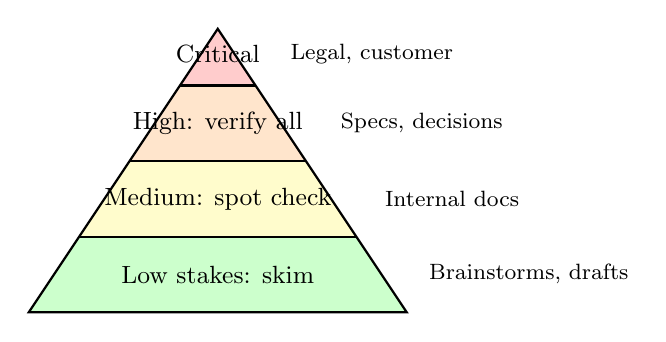
\begin{tikzpicture}[scale=0.8]
% Pyramid layers
\fill[green!20] (-3, 0) -- (3, 0) -- (2.2, 1.2) -- (-2.2, 1.2) -- cycle;
\fill[yellow!20] (-2.2, 1.2) -- (2.2, 1.2) -- (1.4, 2.4) -- (-1.4, 2.4) -- cycle;
\fill[orange!20] (-1.4, 2.4) -- (1.4, 2.4) -- (0.6, 3.6) -- (-0.6, 3.6) -- cycle;
\fill[red!20] (-0.6, 3.6) -- (0.6, 3.6) -- (0, 4.5) -- cycle;

% Outlines
\draw[thick] (-3, 0) -- (3, 0) -- (0, 4.5) -- cycle;
\draw[thick] (-2.2, 1.2) -- (2.2, 1.2);
\draw[thick] (-1.4, 2.4) -- (1.4, 2.4);
\draw[thick] (-0.6, 3.6) -- (0.6, 3.6);

% Labels
\node[font=\small] at (0, 0.6) {Low stakes: skim};
\node[font=\small] at (0, 1.8) {Medium: spot check};
\node[font=\small] at (0, 3) {High: verify all};
\node[font=\small] at (0, 4.1) {Critical};

% Right side annotations
\node[font=\footnotesize, right] at (3.2, 0.6) {Brainstorms, drafts};
\node[font=\footnotesize, right] at (2.5, 1.8) {Internal docs};
\node[font=\footnotesize, right] at (1.8, 3) {Specs, decisions};
\node[font=\footnotesize, right] at (1, 4.1) {Legal, customer};
\end{tikzpicture}%
}

% ============================================
% FIGURE: Three Convergences
% ============================================
\newcommand{\figThreeConvergences}{%
\begin{tikzpicture}[
    circle node/.style={circle, draw=blue!60!black, fill=blue!10, minimum size=2.5cm, align=center, font=\small}
]
% Three circles in Venn-like arrangement
\node[circle node] (compute) at (0, 1.5) {Compute\\became\\cheap};
\node[circle node] (data) at (-1.8, -1) {Data\\became\\abundant};
\node[circle node] (interface) at (1.8, -1) {Interface\\became\\human};

% Center label
\node[font=\bfseries, blue!80!black] at (0, 0) {2022-23};

% Arrows pointing to center
\draw[-{Stealth}, thick, gray] (compute.south) -- (0, 0.5);
\draw[-{Stealth}, thick, gray] (data.east) -- (-0.3, -0.2);
\draw[-{Stealth}, thick, gray] (interface.west) -- (0.3, -0.2);
\end{tikzpicture}%
}
